We next consider a complex entire-muscle model involving motoneurons, sarcomeres and spindles.
The motoneurons and sarcomeres are used to model a \e{motorunit}, which is associated with a specific \e{fibre type} $\tau\in[0,1]$.
Here, $\tau=0$/$\tau=1$ corresponds to slow/fast twitch fibres, respectively.
We choose $\mups\in \N$ different motorunits in a ``motorunit-pool'', specified by $\tau_k\in[0,1], k=1\ldots\mups$.

\subsection{Motoneuron}\label{sec:motoneuron}
The motoneuron model \cite{Cisi2008, negro2011} consists of $6$ degrees of freedom and reads as
\begin{align}
	\vq'(t) &= \fmo(\vq(t),\tau) + \ve_2\kappa(t)\eta(t,\tau) + \ve_2\eta_b(t) & \vq(0) &= \vnull,\label{def:motosys}
\end{align}
for any fibre type $\tau$.
Here, $\ve_2\in\R^6$ is the second unit-vector, $\eta(t,\tau),\eta_b(t)$ describe noises (fibre-type dependent and base noise)
and $\kappa(t)$ an external input signal (e.g. from the central cortex).
This is used to activate/stimulate the motoneuron by addition to the second component $\fmo_2$, which describes the voltage change on the cell's soma.
The external signal $\kappa(t)$ can be seen as a \e{mean current}, as it imitates the overloaded signal from many firing distant neurons.
We will use $\vq^k(t) \in \R^6$ to indicate the current state of the $k$-th motoneuron (of the $k$-th motorunit).

\fix{motoneuron model parameter interpolation (coolExp)}
\fix{maximum mean input current!}

\subsection{Sarcomere}
The sarcomere model describes the force development inside a muscle fibre and is taken from \cite{Shorten2007}.
It has $56$ degrees of freedom and is given by
\begin{align}
	\vr'(t) &= \fsa(\vr(t),\tau) & \vr(0) &= \vr_0(\tau),\label{def:sarcosys}
\end{align}
for any fibre type $\tau$.
There is a set of $105$ (fibre-type dependent) constants for the model, which we denote by $\csa(\tau)\in\R^{105}$.
We denote by $\vr^k(t)\in\R^{56}$ the state of the $k$-th sarcomere model (of the $k$-th motorunit).

\subsection{Spindle}
The spindle is the muscle component responsible for motoneuron feedback, where the model used is from \cite{Mileusnic2006}.
It has $9$ degrees of freedom and is given by
\begin{align}
	\vs'(t) &= \fsp(\vs(t),\dla(t),\nu(t)) & \vs(0) &= \vnull,\label{def:spindlesys}
\end{align}
where $\dla$ describes the change in fibre length and $\nu$ the frequency of an associated motoneuron.
We denote by $\vs^k(t)\in\R^9$ the state of the $k$-th spindle model. In real muscles, the number of spindles is independent from the
number of motorunits, but we use $\mups$ here for simplicity.

\subsection{Model connections}
As the models have not been primarily designed to be used in a compound, we needed to develop appropriate means for their connection.
In this Section we will detail how the different models have been connected.
Figure \ref{fig:modelconn} shows an illustration of the overall model interaction and information flow.
%
\begin{figure}[!htp]
    \begin{center}%
    \begin{tikzpicture}[auto,%
            block_assign/.style ={rectangle, draw=black, very thick, fill=white,%
            text width=10em, text centered, minimum height=3em, inner sep=6pt},%
            block_big/.style ={rectangle, draw=black, very thick, fill=white,%
            text width=14em, text centered, minimum height=3em, inner sep=6pt},%
            block_dashed/.style ={rectangle, draw=black, very thick, fill=white,%
            text width=10em, text centered, minimum height=3em, inner sep=6pt},%
        ]%
        \tikzstyle{stateEdgePortion} = [black, very thick, -latex', shorten >=1pt];
        \tikzstyle{stateEdge} = [stateEdgePortion];
        \tikzstyle{edgeLabel} = [pos=0.5, text centered];
        \tikzstyle{edgeLabelLow} = [pos=0.25, text centered];
        \tikzstyle{edgeLabelHigh} = [pos=0.25, text centered];
        \tikzstyle{line} = [draw, black, very thick, -latex', shorten >=1pt]];
        \tikzstyle{sline} = [draw, black, very thick];
        \tikzstyle{dline} = [draw, black, dashed, very thick, -latex', shorten >=1pt]];
        \tikzstyle{doublearrow} = [draw, black, very thick, <->, -latex', shorten >=1pt, shorten <=5pt, >=stealth]];
%        \tikzstyle{doubledline} = [draw, black, dashed, very thick, <->, -latex', shorten >=1pt, shorten <=5pt, >=stealth]];
        \node [block_big] (neuro)  {{\bf motoneurons} $\vq^k(t)$\\firing times, spindle feedback};%
        \node [block_big, below of=neuro, node distance=30mm] (cell)  {{\bf half-sarcomeres $\vr^k(t)$}\\ action potential, active stress};%
        \node [block_big, above of=neuro, node distance=30mm] (ext)  {{\bf External signal}\\ Control, central cortex};%
        \node [block_dashed, left of=cell, node distance=80mm] (spindle)  {{\bf spindles $\vs^k(t)$} \\ electrical feedback};%
        \node [block_big, below of=cell, node distance=30mm] (mechanics)  {{\bf 3D continuum mechanics $\vu(t),\vv(t),\vw(t)$} \\ geometry, deformation};%
        \path [line] (neuro) -- (cell) node[edgeLabel]{$q^k_2(t)$};
        \draw (cell.south) edge[stateEdge] node[edgeLabel]{$\alpha(X,t)$} (mechanics.north);
        \path [line] (mechanics) -| (spindle) node[edgeLabelHigh]{$\dla(X_k,t),\la''(X_k,t)$};
    	\path [line] ($(neuro.west) + (0,0.3)$) -| ($(spindle.north) + (-0.5,0)$);
    	\path [line] ($(spindle.north) + (0.5,0)$) |- ($(neuro.west) + (0,-0.3)$);
    	\path [line] (ext) -- (neuro.north) node[edgeLabel] {$\kappa(t),\eta(t),\eta_b(t)$}; 
      	\node at (-5.7,-0.7) {$\kappa^s(t)$};
    	\node at (-5.8,0.8) {$\kappa(q^k_2(t))$};
    \end{tikzpicture}%
    \end{center}%
    \caption{Illustration of model connections and interaction}
    \label{fig:modelconn}
\end{figure}

\subsubsection{Motoneuron to Sarcomere}
The motoneuron soma signals $q^k_2(t)$ are used to provide activation spikes for the $k$-th sarcomere.
As the sarcomere model merely reacts to high spikes, the motoneuron output is scaled by a nonlinear function $\gamma$ to emphasize high peaks.
Essentially, the small signals are multiplied by a small factor $\beta_m = 0.3$, and the high signals are intensified by $\beta_M = 7$.
The transition from low to high factor is realized by a smooth Gaussian,
where we choose a threshold signal of $q_M = 40$ to pinpoint the signal from which on the $\beta_M$ factor is applied:
\begin{align}
	\gamma(q) &:= \begin{cases}
		\beta_m + e^{-(q-q_M)^2/150}(\beta_M-\beta_m), & 0 < q < q_M\\
		\beta_M & q \geq q_M,
	\end{cases}
\end{align}
Figure \ref{MSLink} illustrates the 
\begin{figure}[!ht]
	\centering
	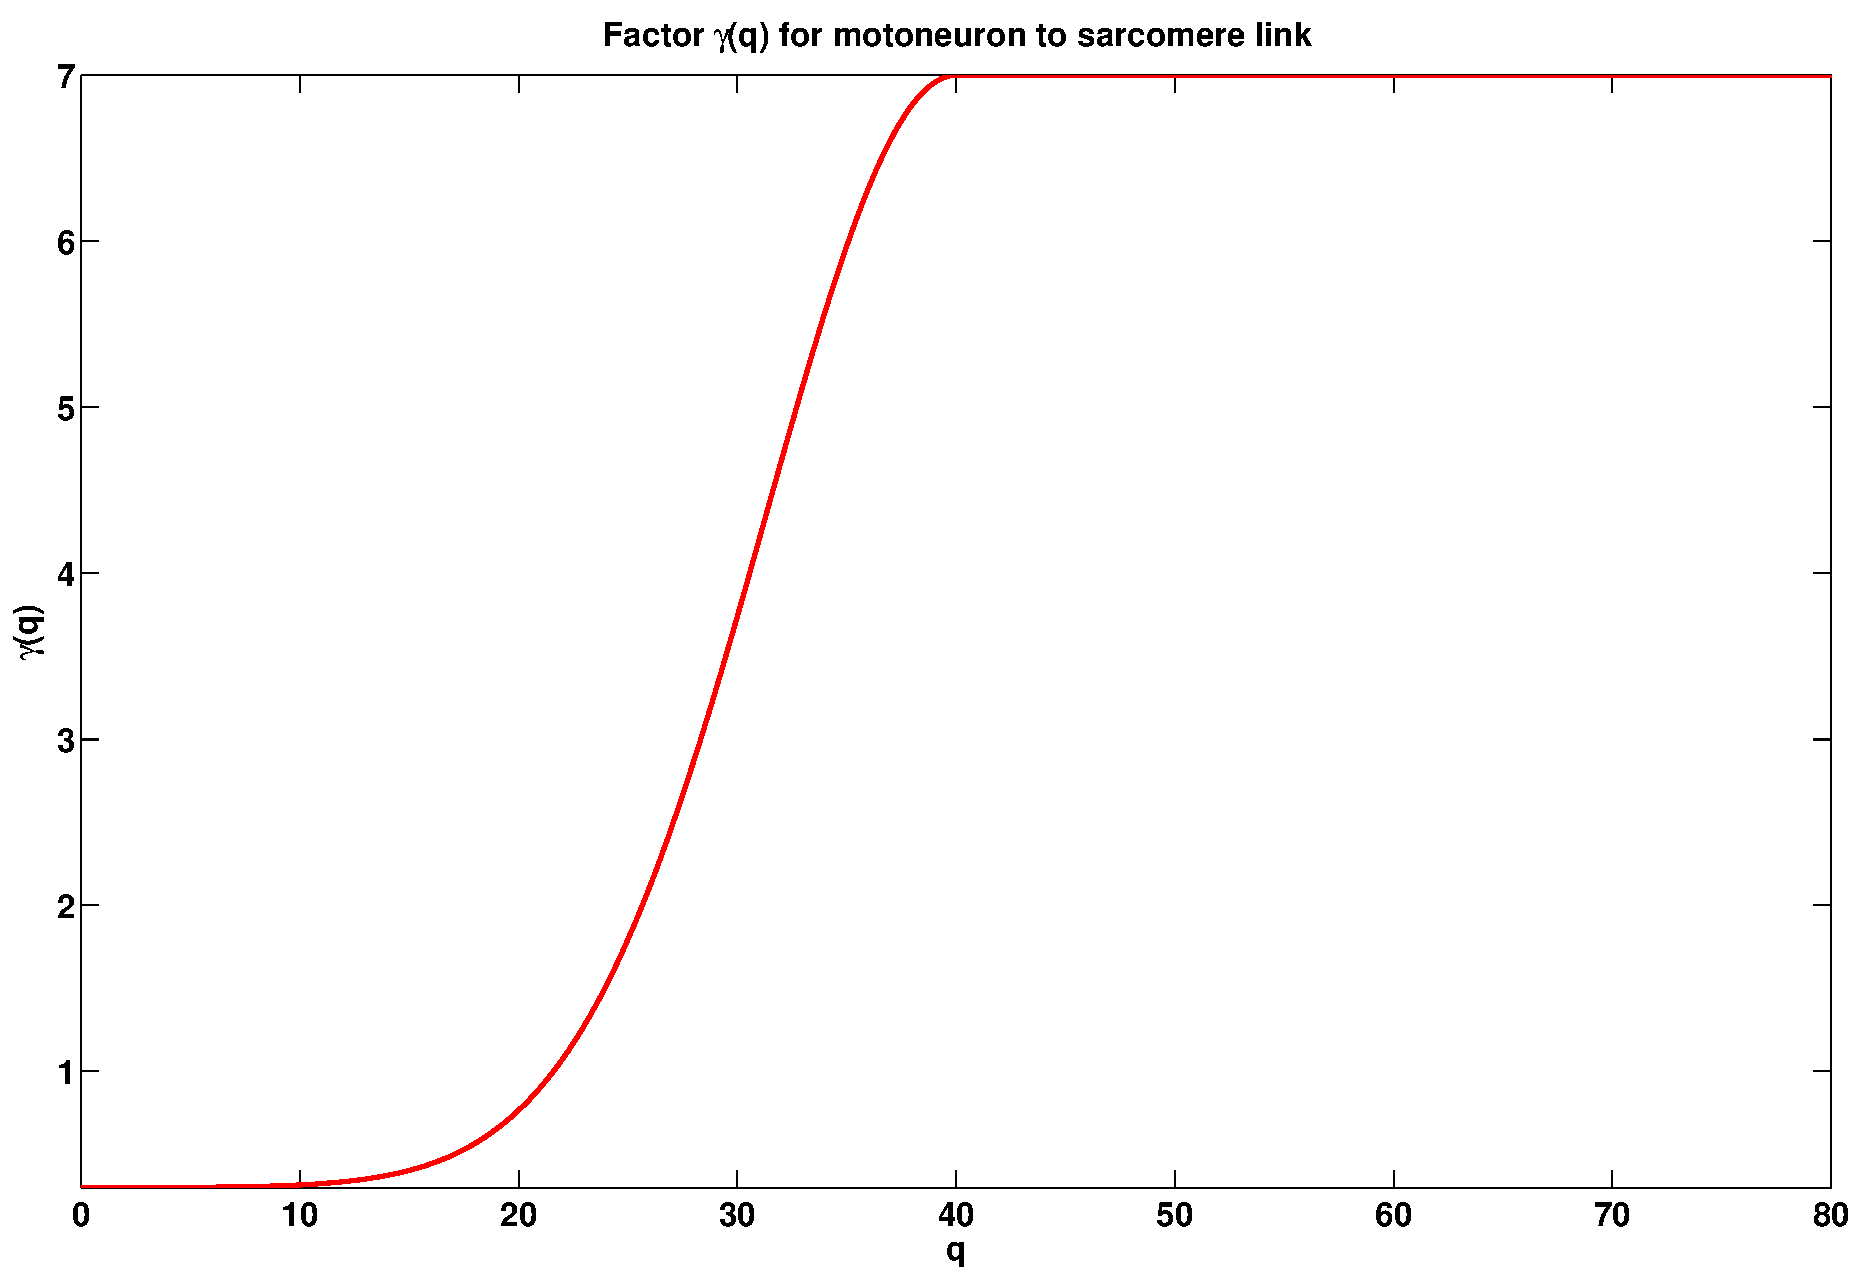
\includegraphics[width=\single]{moto_sarco_link_factor.pdf}
	\caption{Amplification factor for motoneuron signals}
	\label{fig:MSLink}
\end{figure}
Taking into account division by sarcomere model constants, the sarcomere models now read as
\begin{align}
	{\vr'}^k(t) &= \fsa(\vr^k(t),\tau_k) + \ve_1 \frac{\gamma(q_2^k(t))}{\csa_1(\tau_k)}q_2^k(t),\label{def:sarcosys_plus_moto}
\end{align}
where $\ve_1 \in \R^{56}$ denotes the first unit vector, i.e. the signal is added to the first component of the sarcomere models.

\subsubsection{Sarcomere to Mechanics}
The sarcomere model component $r_{53}^k(t)$ is an indicator for the currently developed force in the muscle fibre.
\fix{hier das modell aus der diss erwähnen mit fasern und diffusion + erläuterung}
Within the mechanics FE-framework, this can be transformed to active stress $\alpha(X,t)$ in $\vSf$ by weighting of all $\mups$ force signals at spatial locations.
Hence, we make the ansatz
\begin{align}
	\alpha(X,t) = \sum\limits_{k=1}^\mups w_k(X)\frac{r^k_{53}(t)-r^k_0}{r^k_M}.\label{def:alpha}
\end{align}
Here, we introduce weight functions $w_k(X)$ for the fibre forces satisfying $\sum w_k(X) = 1 \fo X$.
Further, the constants $r_0^k$ denote the base-line level of the $53$rd component and
$r^k_M\in\R$ are the maximum forces for each motorunit (i.e. $\tau_k$), determined by a long-time simulation of each sarcomere model using an
artificial $60Hz$ stimulation.
This ensures that $\alpha(X,t) \in [0,1] \fo X,t$. 

\subsubsection{Mechanics to Spindle}
According to \ref{def:spindlesys}, the spindle models use two external inputs:
The current change rate $\dla$ of fibre stretch and the motoneuron frequency $\kappa(t)$, where the latter will be discussed in Section
\ref{subsec:moto_spindle}.
As the fibre stretch is a local property of the continuum, we fix $\mups$ spindle locations $X_k\in\Omega$ and simply observe $\dla(X_k,t)$ to obtain the second
argument of the $k$-th spindle dynamics $\fsp$.
We recall the definition \eqref{def:fibrestretch} and observe 
\begin{align}
	\dla(X,t) &= \d{}{t}\no{\vF(X,t)\va_0(X)} = \frac{(\vF(X,t)\va_0(X))^T}{\no{\vF(X,t)\va_0(X)}}\d{}{t}\vF(X,t)\va_0(X)\nonumber\\
	  &= \frac{1}{\la(X,t)}\va_0(X)^T\vF(X,t)^T\dot{\vF}(X,t)\va_0(X).\label{eq:dlambda}
\end{align}
Hence, if the $X_k$ are chosen among the set of all elements' Gauss integration points, quantities to compute $\dla$ are readily available during mechanics evaluation.

\subsubsection{Spindle to Motoneuron}
According to \cite{Mileusnic2006}, the spindle model has two algebraic scalar quantities called \e{primary} and \e{secondary afferents},
denoted by $\theta_p(\vs^k(t))$ and $\theta_s(\vs^k(t))$, respectively.
These afferents describe the firing frequency in [pps] of the spindle dendrites leading back into the motoneuron pool.
In a muscle, all spindles are connected to the entirety of the motoneuron pool \fix{ref?}, which will be modeled via averaging of all $\mups$ spindle's afferent outputs.
This gives a \e{mean spindle activation} of
\begin{align}
	\kappa^s(t) &:= \frac{1}{\mups}\sumjmups w_p\theta_p(\vs^j(t)) + w_s\theta_s(\vs^j(t))
\end{align}
which is added to the change rate of each motoneuron's soma alike the external mean current:
\begin{align}
	\dot{\vq}(t) &= \fmo(\vq(t),\tau) + \ve_2(\kappa(t) + \kappa^s(t))\eta(t,\tau) + \ve_2\eta_b(t).\label{def:motosys_plus_spindle}
\end{align}    
% [6{:}8] , where the \ML-like notation indicates which components of the spindle states $\vs$ are used as arguments.

\subsubsection{Motoneuron to Spindle}\label{subsec:moto_spindle}
In order to provide the Spindle model with the current motoneuron frequency, the discrete signal $s_n := q^k_2(t_n)$ at times $t_n, t_1 < t_2 < t_3 \ldots$ needs to be converted to
a frequency $\nu_n$.
Essentially, the last $W \in\N$ peaks are tracked and the frequency is determined by the time elapsed between the last $W$ peaks.    
This is done by a simple automata described in Figure \ref{fig:FD}, where we have two thresholds $p^+,p^-$ denoting the start and end of a peak, respectively.
\begin{figure}[!ht]
    \centering
	\begin{tikzpicture}[shorten >= 2pt, node distance=2cm, auto]
		\node (S) at (-.5,0) {start};
		\node[state] (poff) at (1,0) {$P_-$};
		\node[state] (pon) at (4,0) {$P_+$};
		\path[->] (S) edge node {} (poff)
				  (poff) edge[out=40,in=140] node[above] {$s_n > p^+$} (pon)
				  (pon) edge[out=40,in=320,looseness=4] node[right] {$s_n > p^-$} (pon)
				  (pon) edge[out=220,in=320] node[below] {$s_n < p^-$} (poff);
	\end{tikzpicture}
    \caption{Frequency-detection automata}\label{fig:FD}
\end{figure}
Whenever the transition from $P_-$ to $P_+$ is done, the ``peak counter'' $k$ (starting from $k=0$) is increased by one and the current time $t_n$ is stored via $t^p_k = t_n$.
Then the frequency sequence is then given by
\begin{align}
	\nu_n &:= \begin{cases}
		\frac{W}{t_n - t^p_{k-W}} & k \geq W,\\
		0 & k < W.
	\end{cases}\label{def:FD_freq}
\end{align}
As the detector essentially computes a local average over $W$ peaks, a larger ``window size'' $W$ improves accuracy with respect to a noisy signal,
while a smaller $W$ renders the detector more sensitive to quick frequency changes.
In our applications $W=3$ or $W=4$ turned out to be appropriate choices.

Alternatively, as the frequency detector has a window-size dependent delay, the resulting motoneuron frequency for any given fibre type and 
mean current can be approximated by a machine learning approach \cite{Wirtz2013a}.
Essentially, collected frequencies $\nu_l$ for parameter pairs $(\tau_l,\kappa_l), l = 1\ldots L$ are used as training data
and the approximation is build to have $\nu \approx \tnu(\tau,\kappa)$ for a new, previously unknown pair $(\tau,\kappa)$ and actual frequency $\nu$.
The left image of Figure \ref{fig:motofreq} shows the raw frequency data measured by the frequency detector described above for a sufficiently long run-time using a suitable training set.
The data is then smoothed by multiple 2D-convolution and learned by the VKOGA algorithm using Wendland kernels \cite{Wirtz2013a, Wirtz2013, Wendland2005}.
Figure \ref{fig:motofreq} shows the smoothed frequency responses and the learned surface.
\begin{figure}[!ht]
	\centering
	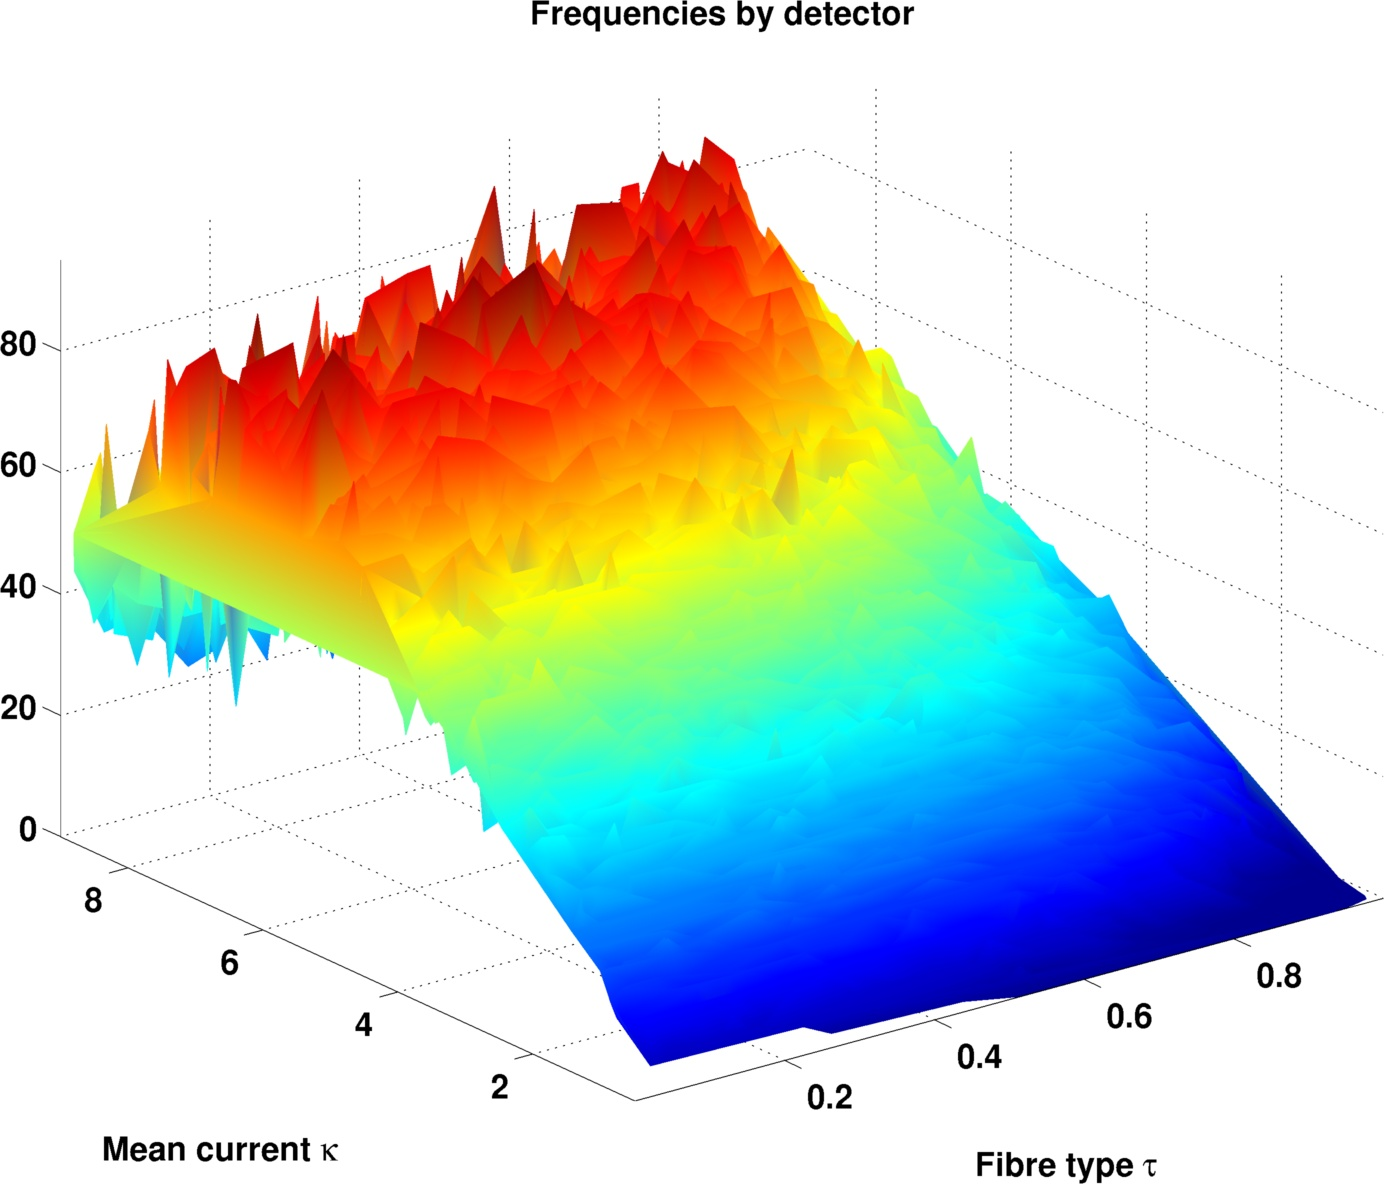
\includegraphics[width=\third]{freq_raw_data}
	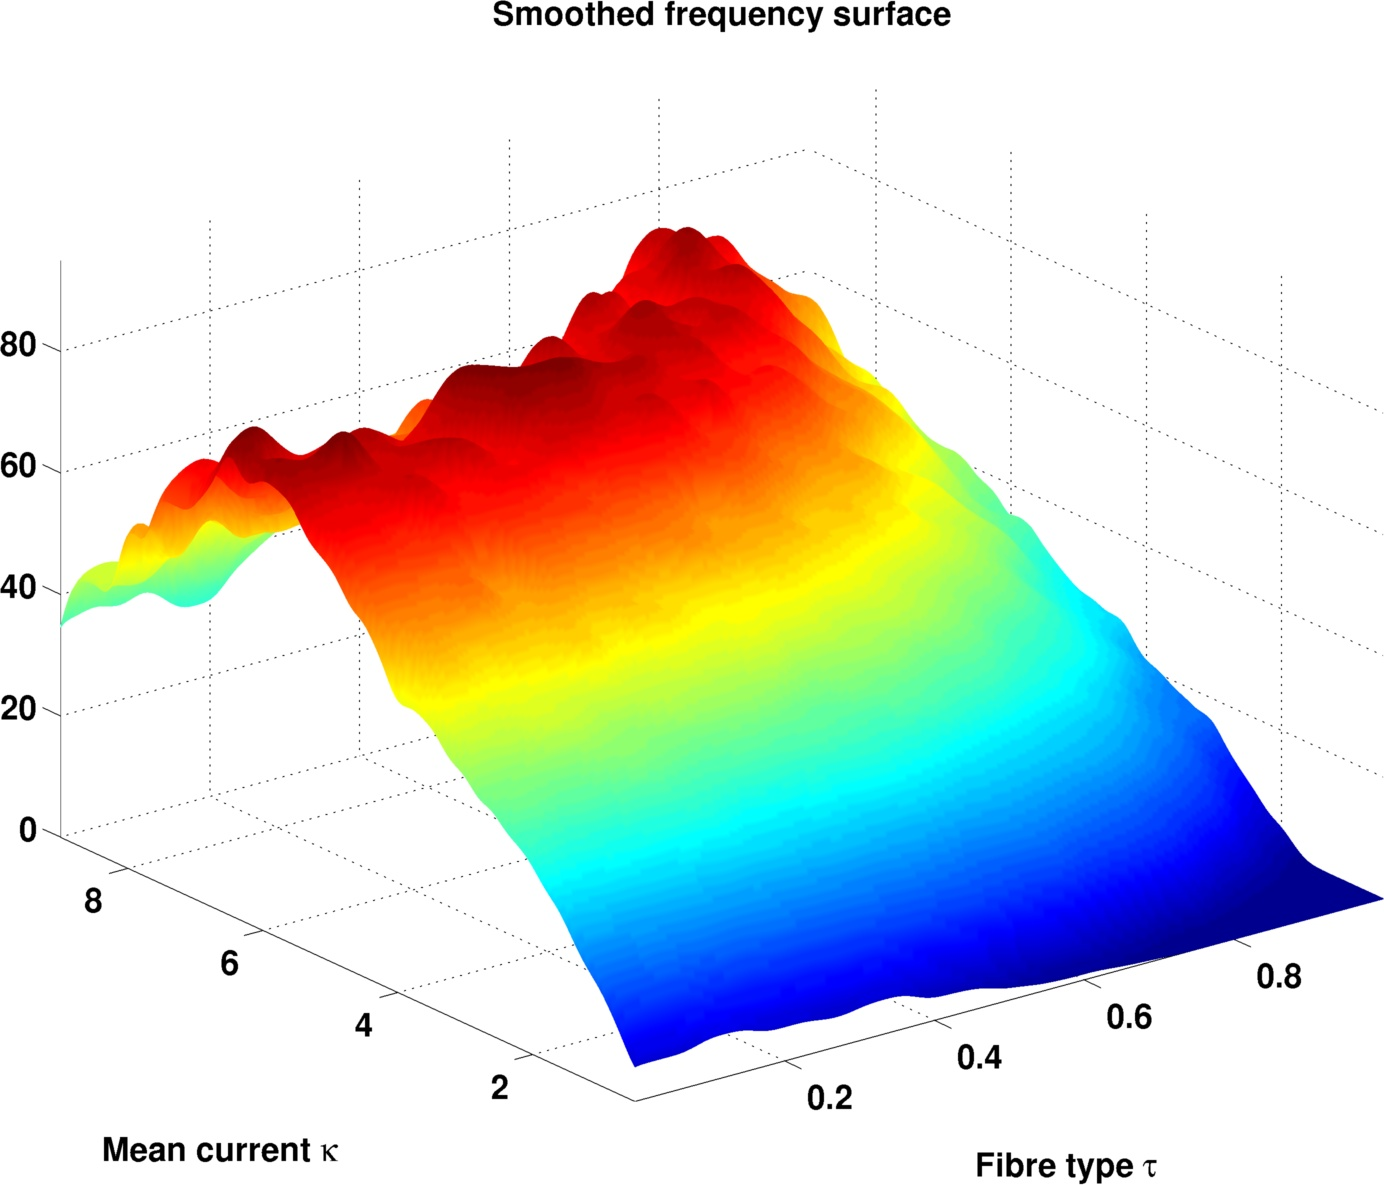
\includegraphics[width=\third]{freq_smoothed}
	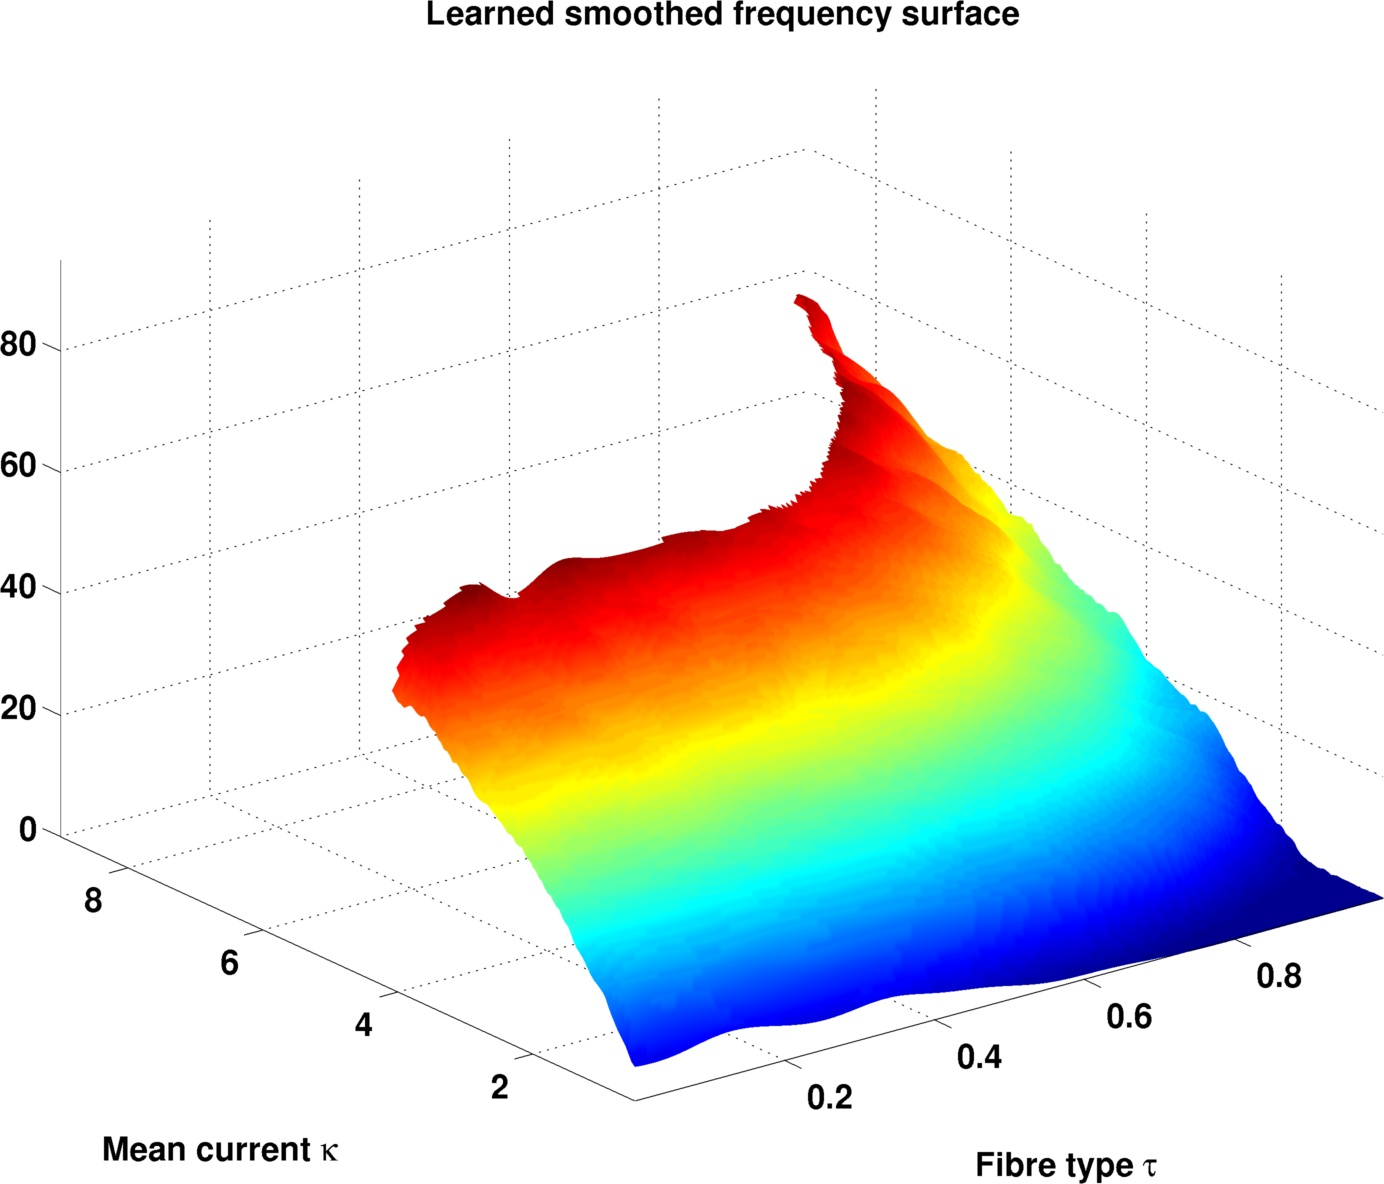
\includegraphics[width=\third]{freq_approx}
	\caption{Frequency response of Motoneurons in Hz for different fibre types $\tau$ and mean currents $\kappa$.
	Left: Raw data, center: smoothed data, right: Learned response surface (cut to the region of valid inputs, see Section \ref{sec:motoneuron})}
	\label{fig:motofreq}
\end{figure}
Mathematically, the VKOGA yields a kernel expansion
\begin{align}
	\tnu(\vz) &= \suml{j=1}{C}c_j\Phi(\vz,\vz_j), & c_j &\in \R,  & \vz_j\in\R^2. 
\end{align}
Here, the kernel $\Phi$ is a Wendland kernel given by
\begin{align}
	\Phi(\vz,\tilde{\vz}) &= \phi\left(\frac{\noG{\vz-\tilde{\vz}}}{\gamma}\right), & \phi(r) &= (1-r)^{l+k}_+p(r),\\
	p(r) &= \frac{1}{3}(l^2 + 4l + 3)r^2 + (l + 2)r + 1, & l &:= \lfloor d/2\rfloor + k + 1.
\end{align}
where we used $k=d=2$.
Here, $k$ is a hyperparameter for \e{smoothness} in the sense of $\Phi\in C^{2k}(\Omega)$ if $\Omega \subseteq \R^{\hat{d}}, \hat{d}\leq d$, see \cite{Wendland2005}.

With this, instead of using \eqref{def:FD_freq}, one can obtain the current $k$-th motoneuron frequency as $\tnu(\tau_k,\kappa)$ for given mean current $\kappa$.

\subsubsection{Model parameters}
\begin{table}[!ht]
	\begin{tabular}{l|l|l}
		Name & Value & Context\\\hline
		$\beta_m$ & 0.3 & Moto-Sarco link min factor\\
		$\beta_M$ & 7 & Moto-Sarco link max factor\\
		$q_M$ & 40 & Moto-Sarco link max factor signal\\
		$w_p$ & 0.002 & Primary afferent weight\\
		$w_s$ & 0.002 & Secondary afferent weight\\
		$p^+$ & 40 & Frequency detector ``peak on'' threshold\\
		$p^-$ & 15 & Frequency detector ``peak off'' threshold\\
		$W$ & 3-4 & Frequency detector peak window size
	\end{tabular}
	\caption{Model-related parameters}\label{tab:params}
\end{table}
\begin{table}[!ht]
	\begin{tabular}{l|ll}
		Name & Context\\\hline
		$r^k_M$ & Maximum force response of single sarcomere at constant, full activation ($60Hz$)\\
		$r^k_0$ & Base-line or minimum force response of the $k$-th sarcomere 
	\end{tabular}
	\caption{Experimentally determined quantities}\label{tab:params}
\end{table}
\begin{table}[!ht]
	\begin{tabular}{l|ll}
		Name &  Context\\\hline
		$w_k$ & Weights for fibre forces at each Gauss point  
	\end{tabular}
	\caption{Model design variables}\label{tab:params}
\end{table}

\subsection{Overall dynamical system}
In this section we detail the numerical implementation of the overall connected model as system of ODEs.
The muscle activation introduced in Section \ref{sec:active_force} now is computed using the sarcomere states $\vr^k$.
This renders the stress tensor \eqref{def:completeP} and hence the operator $K$ from \eqref{def:Kop} dependent of $\vr^1(t),\ldots,\vr^\mups(t)$,
so we write $K(\vu(t),\vw(t),\vr^1(t),\ldots,\vr^\mups(t))$.
Moreover, the motoneurons \eqref{def:motosys} receive feedback from all spindles via $\kappa^s(\vs^1(t),\ldots,\vs^\mups(t))$.
%As each sarcomere is linked to its motoneuron, the sarcomere dynamics \eqref{def:sarcosys} now read as $\fsa(\vr^k(t),\tau_k,\vq^k(t))$.
The spindles \ref{def:spindlesys} receive lambda stretch information $\dla(X_k,t)$ from the mechanics model at locations $X_k$.
Recalling \eqref{eq:Fdependencyrewrite} and the substitution $\vv(t) = \vu'(t)$ from Section \ref{sec:odeform} we see that similarly
\begin{align}
	\dot{\vF}(X,t) &= \sumi \vc'_i(t)\otimes \nabla\varphi_i(X) = \sumi \vv[i](t)\otimes \nabla\varphi_i(X) =: \dot{\vF}(X,\vv(t)).\label{eq:Fdotdependencyrewrite}
\end{align}
Hence, by virtue of \eqref{eq:dlambda}, we see that $\dla(X,t) =: \dla(X,\vu(t),\vv(t))$, which finally gives $\fsp(\vs^k(t),\vu(t),\vv(t))$.

Finally, using the above, \eqref{def:motosys_plus_spindle} and \eqref{def:sarcosys_plus_moto}, the overall system \eqref{def:mainsys} can be extended to
\begin{align}%\label{def:mainsys_full}
	\dot{\vu}(t) &= \vv(t)\\
	\vM\dot{\vv}(t) &= -K(\vu(t),\vw(t),\vr^1(t),\ldots,\vr^\mups(t)) - \vD\vv(t)\\
		& \vdots\nonumber\\
	\dot{\vq}^k(t) &= \fmo(\vq^k(t),\tau_k) + \ve_2^9(\kappa(t) + \kappa^s(\vs^1(t),\ldots,\vs^\mups(t)))\eta(t,\tau) + \ve_2^9\eta_b(t)\\
		 & \vdots\nonumber\\
	\dot{\vr}^k(t) &= \fsa(\vr^k(t),\tau_k) + \ve^{56}_1 \frac{\gamma(q_2^k(t))}{\csa_1(\tau_1)}q_2^k(t)\\
		& \vdots\nonumber\\
	\dot{\vs}^k(t) &= \fsp(\vs^k(t),\vu(t),\vv(t))\\
		& \vdots\nonumber\\
% 	\dot{\vq}^1(t) &= \fmo(\vq^1(t),\tau_1) + \ve_2(\kappa(t) + \kappa^s(\vs^1(t),\ldots,\vs^\mups(t)))\eta(t,\tau) + \ve_2\eta_b(t)\\
% 		\vdots &= \vdots\nonumber\\
% 	\dot{\vq}^\mups(t) &= \fmo(\vq^\mups(t),\tau_\mups) + \ve_2(\kappa(t) + \kappa^s(\vs^1(t),\ldots,\vs^\mups(t)))\eta(t,\tau) + \ve_2\eta_b(t)\\
% 	\dot{\vr^1}(t) &= \fsa(\vr^1(t),\tau_1) + \ve_1 \frac{\gamma(\vq_2^1(t))}{\csa_1(\tau_1)}\vq_2^1(t)\\
% 		\vdots &= \vdots\nonumber\\
% 	\dot{\vr^\mups}(t) &= \fsa(\vr^\mups(t),\tau_\mups) + \ve_1 \frac{\gamma(\vq_2^\mups(t))}{\csa_1(\tau_\mups)}\vq_2^\mups(t)\\
% 	\dot{\vs^1}(t) &= \fsp(\vs^1(t),\vu(t),\vv(t))\\
% 		\vdots &= \vdots\nonumber\\
% 	\dot{\vs^\mups}(t) &= \fsp(\vs^\mups(t),\vu(t),\vv(t))\\
	\text{s.t.}\quad \vg(\vu(t))		&= \vnull.
\end{align}

\subsubsection{Derivation of $\nabla_{\vr^k}K(\vu(t),\vw(t),\vr^1(t),\ldots,\vr^\mups(t))$}
For any $k = 1\ldots\mups, j=1\ldots N$ we have similar to \eqref{def:dKduji}
\begin{align}
	\d{K[j]}{r^k_i}(\vu,\vw,\vr^1,\ldots,\vr^\mups) &= \sumvk\sumgp w_p \d{\vPnl}{r^k_i}(\pmp,\vu,\vw,\ldots,\vr^k,\ldots) \dNjmp\jmp\\
	\d{\vPnl}{r^k_i}(\ldots,\vr^k,\ldots) & \re{def:completeP} \d{}{r^k_i} g(\la(\pmp,\vu),\dla(\pmp,\vu,\vv),\alpha(\pmp,\vr^1,\ldots,\vr^\mups))\nonumber\\
	&\qquad\cdot\vF(\pmp,\vu)\va_0(\pmp)\otimes\va_0(\pmp)\\
	&= \d{g}{\alpha}(\la(\pmp,\vu),\dla(\pmp,\vu,\vv),\alpha)\d{\alpha}{r^k_i}(\pmp,\vr^1,\ldots,\vr^\mups)\nonumber\\
	&\qquad\cdot\vF(\pmp,\vu)\va_0(\pmp)\otimes\va_0(\pmp)\\
	\d{g}{\alpha}(\la,\dla,\alpha) &\re{def:g} \frac{p^{max}}{\la}f_l(\la)f_v(\dla)\\
	\d{\alpha}{r^k_i}(\pmp,\vr^1,\ldots,\vr^\mups) &\re{def:alpha} \d{}{r^k_i}\sum\limits_{l=1}^\mups w_l(\pmp)\frac{r^l_{53}(t)-r^l_0}{r^l_M} = \begin{cases}
		\frac{w_k(\pmp)}{r^k_M} & i=53\\
		0 & \text{else}
	\end{cases}
\end{align}
\begin{align}	
	\Rightarrow\d{K[j]}{r^k_{53}} &= \sumvk\sumgp w_p \Biggl(\frac{p^{max}}{\la(\pmp,\vu)}f_l(\la(\pmp,\vu))f_v(\dla(\pmp,\vu,\vv))\frac{w_k(\pmp)}{r^k_M}\nonumber\\
	&\qquad \cdot \vF(\pmp,\vu)\va_0(\pmp)\otimes\va_0(\pmp)\dNjmp\jmp\Biggr),\\
	\d{K[j]}{r^k_i} &= 0 \qquad i \neq 53
\end{align}

\subsubsection{Moto to Sarco Jacobian}
\begin{align}
	\d{}{q_2^k}\dot{r}_1^k(\vr^k,\tau_k) &= \d{}{q_2^k}\frac{\gamma(q_2^k)}{\csa_1(\tau_k)}q_2^k = \frac{\gamma(q_2^k)}{\csa_1(\tau_k)} + \frac{q_2^k}{\csa_1(\tau_k)}\d{}{q_2^k}\gamma(q_2^k)\\
	&=  \frac{\gamma(q_2^k)}{\csa_1(\tau_k)} - \frac{q_2^k(q_2^k-q_M)}{\csa_1(\tau_k)75}e^{-(q_2^k-q_M)^2/150}(\beta_M-\beta_m)
\end{align}

\subsubsection{Spindle to Moto}
\begin{align}
	\d{}{s^k_i}\dot{\vq}(t) &= \d{}{s^k_i}\ve_2(\kappa(t) + \kappa^s(\vs^1,\ldots,\vs^\mups))\eta(t,\tau)\\
	&= \ve_2\eta(t,\tau)\d{}{s^k_i}\kappa^s(\vs^1,\ldots,\vs^\mups)\\
	&= \ve_2\frac{\eta(t,\tau)}{\mups}\d{}{s^k_i}\sumjmups w_p\theta_p(\vs^j) + w_s\theta_s(\vs^j)\\
	&= \ve_2\frac{\eta(t,\tau)}{\mups}\left(w_p\d{}{s^k_i}\theta_p(\vs^k) + w_s\d{}{s^k_i}\theta_s(\vs^k)\right)
\end{align}

\subsection{Spindle via learned Frequency}
If the learned frequency $\tnu$ is used, the spindle link via the motoneuron leads to an immediate feedback for the spindle dynamics as then
\begin{align}
	\dot{\vs}^k(t) &= \fsp(\vs^k(t),\dla(t),\tnu(t))\\
	&= \fsp(\vs^k(t),\dla(t),\tnu(\tau_k,\kappa(t) + \kappa^s(\vs^1(t),\ldots,\vs^\mups(t))))
\end{align}
Hence we get
\begin{align}
	\d{}{s_i^j}\fsp(\vs^k,\dla,\tnu(\vs^1,\ldots,\vs^\mups)) &= \delta_{jk}\frac{\partial_1}{\partial s_i^j}\fsp(\vs^k,\dla,\tnu)
	 + \frac{\partial_3}{\partial s_i^j}\fsp(\vs^k,\dla,\tnu(\vs^1,\ldots,\vs^\mups))\\
	\frac{\partial_3}{\partial s_i^j}\fsp(\vs^k,\dla,\tnu(\vs^1,\ldots,\vs^\mups))
	&= \d{}{\tnu}\fsp(\vs^k,\dla,\tnu)\d{}{\kappa}\tnu(\tau,\kappa)\d{}{s_i^j}\kappa^s(\vs^1,\ldots,\vs^\mups)
\end{align}
\begin{align}
	[\ldots]&= \d{}{\tnu}\fsp(\vs^k,\dla,\tnu)\suml{l=1}{C}c_l\d{}{\kappa}\Phi((\tau_k,\kappa),\vz_l)
	\frac{1}{\mups}\left(w_p\d{}{s^j_i}\theta_p(\vs^j) + w_s\d{}{s^j_i}\theta_s(\vs^j)\right)
\end{align}

\subsubsection{Mechanics to Spindle}
For $k=1\ldots\mups, j = 1\ldots N, i=1\ldots3$ we have
\begin{align}
	\d{}{\vu[j]_i}\fsp(\vs^k,\dla(X,\vu,\vv),\nu) &= \d{}{\dla}\fsp(\vs^k,\dla,\nu)\d{}{\vu[j]_i}\dla(X,\vu,\vv)\\
	\d{}{\vu[j]_i}\dla(X,\vu,\vv) &\re{eq:dlambda} \d{}{\vu[j]_i}\frac{1}{\la(X,\vu)}\va_0(X)^T\vF(X,\vu)^T\dot{\vF}(X,\vv)\va_0(X)
\end{align}
\begin{align*}
   \d{}{\vu[j]_i} [\ldots] &= \d{}{\vu[j]_i}\left(\frac{1}{\la(X,\vu)}\right)\va_0(X)^T\vF(X,\vu)^T\dot{\vF}(X,\vv)\va_0(X)\\
   &\quad+ \frac{1}{\la(X,\vu)}\d{}{\vu[j]_i}\va_0(X)^T\dot{\vF}(X,\vv)^T\vF(X,\vu)\va_0(X)\\
   &= -\frac{1}{\la(X,\vu)^2}\d{}{\vu[j]_i}\Bigl(\la(X,\vu)\Bigr)\va_0(X)^T\vF(X,\vu)^T\dot{\vF}(X,\vv)\va_0(X)\\
   &\quad+ \frac{1}{\la(X,\vu)}\va_0(X)^T\dot{\vF}(X,\vv)^T\vU_i^j\va_0(X)\\
   &\re{eq:dlamdvu} -\frac{1}{\la(X,\vu)^3}\va_0(X)^T\vF(X,\vu)^T\Bigl(\vU_i^j+\dot{\vF}(X,\vv)\Bigr)\va_0(X)\\
   &\quad+ \frac{1}{\la(X,\vu)}\va_0(X)^T\dot{\vF}(X,\vv)^T\vU_i^j\va_0(X)
\end{align*}
\begin{align}
	\d{}{\vv[j]_i}\fsp(\vs^k,\dla(X,\vu,\vv),\nu) &= \d{}{\dla}\fsp(\vs^k,\dla,\nu)\d{}{\vv[j]_i}\dla(X,\vu,\vv)\\
	\d{}{\vv[j]_i}\dla(X,\vu,\vv) &\re{eq:dlambda} \d{}{\vv[j]_i}\frac{1}{\la(X,\vu)}\va_0(X)^T\vF(X,\vu)^T\dot{\vF}(X,\vv)\va_0(X)\\
		&=\frac{1}{\la(X,\vu)}\va_0(X)^T\vF(X,\vu)^T\d{}{\vv[j]_i}\dot{\vF}(X,\vv)\va_0(X)\\
		&\re{eq:Fdotdependencyrewrite}\frac{1}{\la(X,\vu)}\va_0(X)^T\vF(X,\vu)^T\vU^j_i\va_0(X)
\end{align}

\subsubsection{Model connectivity}
The above partial derivatives constitute the overall system Jacobian matrix.
Figure \ref{fig:jacpattern} illustrates the Jacobian sparsity pattern for an example geometry with $18$ Taylor-Hood elements and $\mups=6$ motorunits and spindles.
\begin{figure}[!ht]
	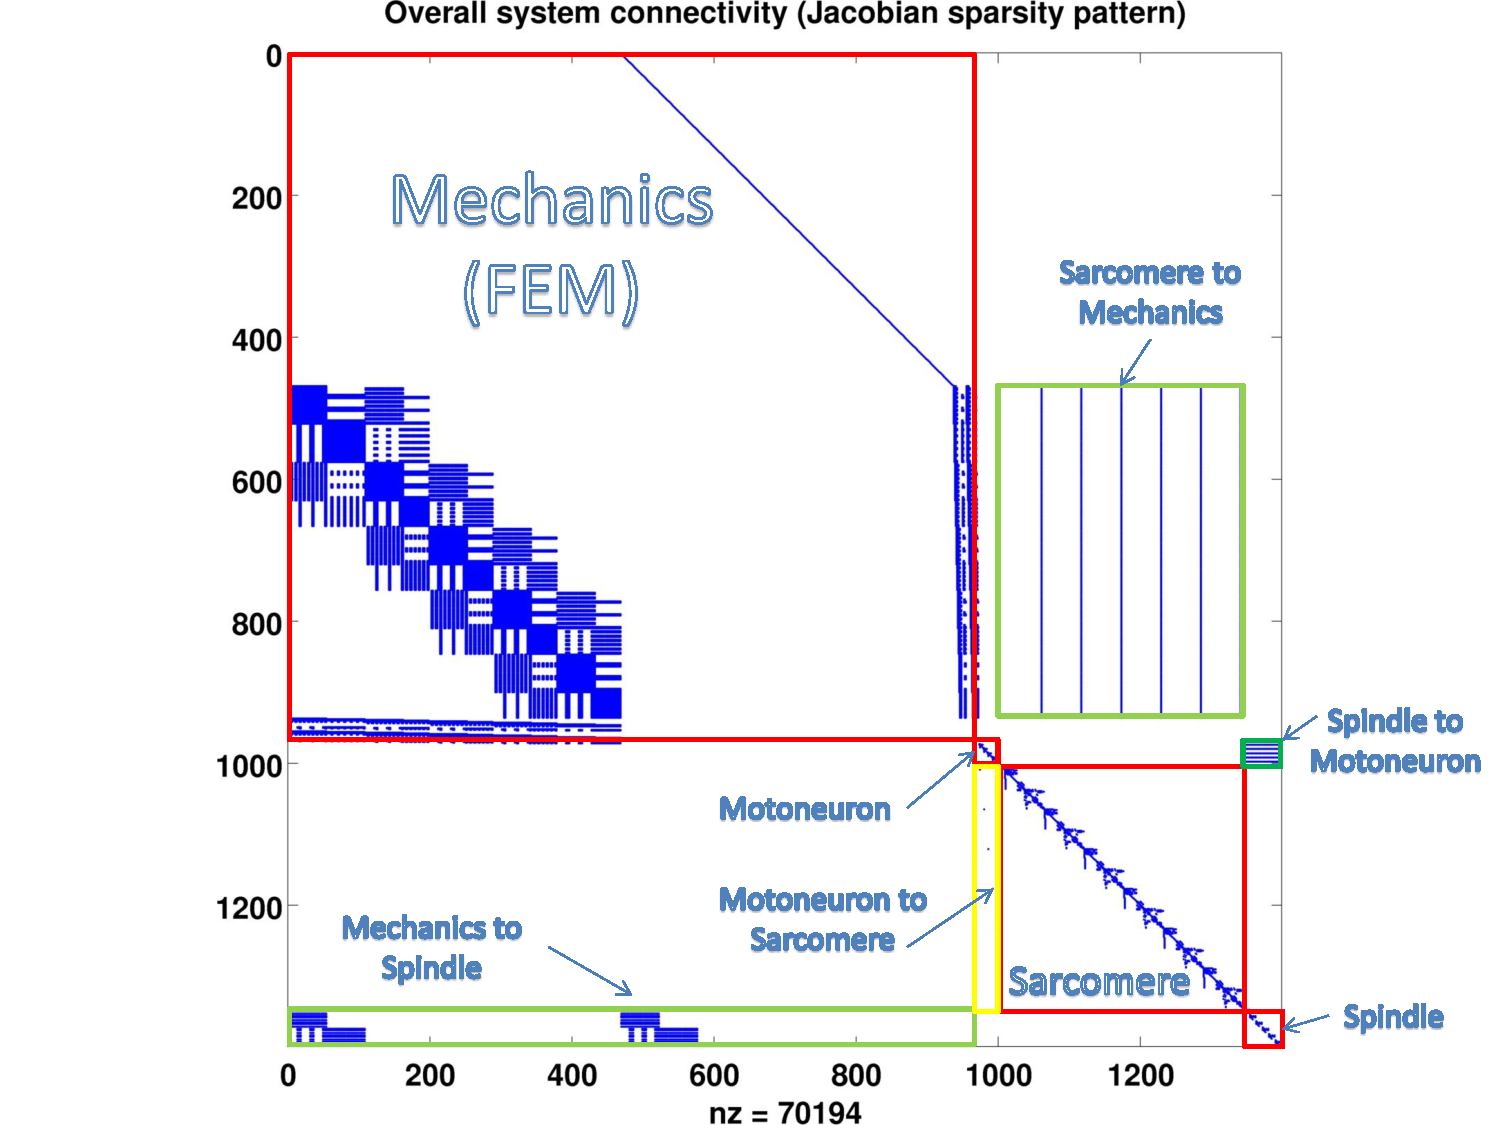
\includegraphics[width=\textwidth]{sparsity_pattern}
	\caption{Jacobian sparsity pattern}
	\label{fig:jacpattern}
\end{figure}
